\documentclass[a4paper,spanish]{article}


\usepackage[spanish]{babel}
\usepackage[latin1]{inputenc}
\usepackage{amsmath}
\usepackage{amssymb}
\usepackage[margin=1.5cm]{geometry}
\usepackage{graphicx}
\usepackage{caption}
\usepackage{subcaption}
\usepackage{float}
\newcommand{\oiint}{\displaystyle\bigcirc\!\!\!\!\!\!\!\!\int\!\!\!\!\!\int}


\usepackage{epsfig}
\usepackage{color}
\usepackage{amsfonts}
\usepackage[T1]{fontenc}

\def\Fou {\mathcal{F}}
\def\Rea {\mathcal{R}e}
\def\Ima {\mathcal{I}m}
\def\N {\mathbb{N}}
\def\C {\mathbb{C}}
\def\Q {\mathbb{Q}}
\def\R {\mathbb{R}}
\def\Z {\mathbb{Z}}


%\renewcommand{\contentsname}{\'Indice}
%\renewcommand{\chaptername}{Cap\'\i tulo}
%\renewcommand{\bibname}{Referencias}

\newtheorem{prop}{Proposici\'on}[section]
\newtheorem{teo}[prop]{Teorema}
\newtheorem{defi}[prop]{Definici\'on}
\newtheorem{obs}[prop]{Observaci\'on}
\newtheorem{cor}[prop]{Corolario}
\newtheorem{lema}[prop]{Lema}
\newtheorem{ejem}[prop]{Ejemplo}
\newtheorem{ejer}[prop]{Ejercicio}

\numberwithin{equation}{section}
\newtheorem{definition}{Definicion}


\newenvironment{proof}{
\trivlist \item[\hskip \labelsep\mbox{\it Demostraci\'on:
}]}{\hfill\mbox{$\square$}
%\trivlist \item[\hskip \labelsep{\sl
%#1}\mbox{Demostraci\'on}]}{\hfill\mbox{$\square$}
\endtrivlist}

%\topmargin 0cm \oddsidemargin 0.7cm %% margenes
%\textheight 21cm \textwidth 15cm %% tamaño del texto
\parindent 0cm %% sangria

\begin{document}

\part{Introducci\'on matem\'atica}

A lo largo de nuestro viaje nos encontraremos y tendremos que amigarnos con los n\'umeros complejos, por lo que es conveniente poder introducirlos ahora con un cierto formalismo para luego
poder referirnos a ellos con comodidad.

\section{El cuerpo $\C$ de los n\'umeros complejos}
Consideremos el conjunto $\R^2$ con las operaciones\\
$$\displaystyle (x,y)+(u,v)=(x+u,y+v)$$
$$\displaystyle (x,y).(u,v)=(xu-yv,xv+yu).$$
Es muy f\'acil comprobar las propiedades asociativa y conmutativa
de las operaciones as\'i­ definidas y la distributiva del producto
respecto de la suma. El elemento neutro de la suma es $(0,0)$ y
$(1,0)$ es la unidad del producto. Adem\'as,
$(-x,-y)$ es el opuesto de $(x,y)$, y
$\forall (x,y) \neq (0,0)$ tiene inverso
\[\displaystyle
(x,y).(\cfrac{x}{x^2+y^2},\cfrac{-y}{x^2+y^2})=(1,0).\] Todas estas
propiedades se resumen en que $(\R^2;+;.)$ es un
$\textit{cuerpo}$, que representamos por $\C$ y les llamamos a sus
elementos n\'umeros complejos.

\subsection{Forma bin\'omica de un numero complejo}

El s\'imbolo usual $\displaystyle(x,y)$ para representar pares
ordenados en la estructura de $\R^2$ como $\R$ espacio vectorial
no es conveniente para representar n\'umeros complejos (calculate
cualquier potencia grande y lo vas a notar). Pero observemos que
\[(x,0)+(y,0)=(x+y,0)\]
\[(x,0).(y,0)=(xy,0).\]

Es decir que los n\'umeros complejos de la forma $(x,0)$ se
comportan respecto a la suma y multiplicaci\'on definidas para los
complejos como n\'umeros reales respecto a su suma y
multiplicaci\'on (O sea $\R\times{\lbrace0\rbrace}$ es un
subcuerpo de $\C$ isomorfo a $\R$). Esto nos permite la
identificaci\'on $\textbf{$(x,0)=x$}$. Por otro lado al n\'umero
complejo $(0,1)$ lo representaremos por $\textit{i}$, la unidad
imaginaria (t\'ermino acu\~nado por Descartes (1596-1650), padre de
los ejes coordenados) y con ello
tenemos\[i^2=(0,1).(0,1)=(-1,0)=-1.\]
Y ahora podemos escribir a todo n\'umero complejo como \\
 \[z=(x,y)=(x,0)+(0,y)=(x,0)+(0,1).(y,0)=x+iy,\]
que le llamamos la forma bin\'omica de un numero complejo donde
$x=\Rea \ z $ y $y=\Ima \ z $
\\
\textbf{Observaci\'on}: Acabamos de ver que $i^2=-1$ pero eso ni
cerca nos permite escribir $i=\sqrt{-1}$, ya que si lo hacemos y
manejamos a la ra\'iz como estamos acostumbrados llegamos a que\\
\[-1=i^2=i.i=\sqrt{-1}.\sqrt{-1}=\sqrt{{-1}.{-1}}=\sqrt{1}=1\]
$\Longrightarrow $-1=1$ \ Abs! $ F\'ijense que en realidad si
escribimos  $i=\sqrt{-1}$ no podemos interpretar a -1 como n\'mero
real (ya que estos no tienen ra\'iz cuadrada de negativos) sino
como $-1$ complejo, por lo que \textit{estamos usando ra\'ices de
n\'umeros complejos sin siquiera haberlas definido y presuponiendo
que mantienen las propiedades de los n\'umeros reales}. Antes de
escribir $i=\sqrt{-1}$ tenemos que saber que significa
$\sqrt{z} \ \forall \ z\in\C$ y ah\'i se ve que
$\sqrt{zw}=\sqrt{z}\sqrt{w}$ generalmente no es v\'alida $\forall \ z,w \in\C\setminus\R^+$.

\textbf{Observaci\'on 2}: No existe un orden en $ \C$! Es
importante remarcar que en los complejos no existe una relaci\'on
de orden como $\leq$ ya que, si la hubiese
\[0<i^2=-1 \Longrightarrow \ 0<1 + {-1} = 0 \ Abs!\]
Por lo tanto hay que tener cuidado con escribir relaciones de
orden en $\C$.

\subsection{M\'odulo y conjugado de un n\'umero complejo}
Dado un n\'umero complejo $z=x+iy$ se puede definir su reflexi\'on
con respecto al eje real pens\'andolo como $\R$ espacio vectorial,
que resulta en el $\textit{conjugado}$ de un n\'umero complejo:
$\overline{z}=x-iy$. Por otro lado tambi\'en en la misma linea de
razonamiento se define el \textit{m\'odulo} de z como $\vert
z\vert=\sqrt{x^2+y^2}$. Intuitivamente se ve al m\'odulo como la
mera norma eucl\'idea, lo que nos lleva a verificar el m\'odulo
cumple las condiciones de una norma y definimos la
\textit{distancia} entre dos n\'umeros complejos como $\vert{z-w}\vert \ \forall \ z,w \in\C$.

\textbf{Propiedades}: Se puede verificar
\begin{enumerate}
\item $\overline{z+w}=\overline{z}+\overline{w}$
\item $\overline{zw}=\overline{z}\overline{w}$
\item $\vert{zw}\vert=\vert {z}\vert.\vert {w}\vert$
\item $\vert {z+w}\vert\leq \vert {z}\vert +\vert {w}\vert$
\end{enumerate}
entre otras. Finalmente vale remarcar

\[z.\overline{z}=\vert{z}\vert^2\]
\[\Longrightarrow \ \forall \ {z} \in \C, z^{-1}=\cfrac{\overline{z}}{\vert{z}\vert^2}\]

\subsection{Forma polar de un n\'umero complejo}
Dado que todo complejo $z=x+iy\neq{0}$ presenta un m\'odulo no
nulo, uno puede escribir
\[z=\vert{z}\vert.\cfrac{x+iy}{\vert{z}\vert}.\] Como el segundo
factor esta en la circunferencia unidad, se tiene que
$\cfrac{x+iy}{\vert{z}\vert}$ tiene una relaci\'on
biun\'ivoca con $\cos{t} + i\sin{t} \ , \ t\in{[0,2\pi)} $. A este $t$
se le llama el \textit{argumento principal} del n\'umero $z$ y
notemos que aunque su definici\'on no acarrea ambiguedades, la
funci\'on $\arg {z} $ resulta discontinua. A la representaci\'on
\[z=r(\cos{\theta}+i\sin{\theta} \ , \ r \in \R^+ \ , \ \theta \in
[0,2 \pi)\] se le llama \textit{forma polar de un n\'umero complejo $z$}.


\section{Exponencial compleja}

Consideremos la serie $\sum\limits_{n\geq{0}} \cfrac{z^n}{n!} $ que, aplicando el criterio del cociente, sabemos que converge para todo $z$ complejo.
Entonces llamamos \textit{exponencial compleja} a la funci\'on \\
\[ \exp{z}= \sum_{n=0} ^{\infty} \cfrac{z^n}{n!} \ \left( z \in \C \right) \]

\subsection{Propiedades}
Se cumplen las siguientes propiedades cuya demostraci\'on, en funci\'on de la definici\'on de la exponencial compleja, no le resultara dificultosa al lector
\begin{enumerate}

\item $exp'(z) = exp (z)$ 
\item $ exp (0) = 1 $
\item $ exp (x)= e^{x} \mbox{ para } \ x \in \R \mbox{  con lo que se justifica } exp (z) = e^{z} \ z \in \C $
\item $ e^{z+w}= e^{z}.e^{w}$
\item $ e^{z} \neq 0 \ \forall \ z \in \C$
\item $ \mbox{ Si } z= x+iy \ \Longrightarrow \ e^{z} = e^{x}.e^{iy} = e^{x}.(\cos(y)+i\sin(y))$

\end{enumerate}
\subsection{Otras funciones complejas \'utiles y forma exponencial}

A partir de la exponencial compleja podemos obtener las funciones seno y coseno complejos, que como se imaginar\'an, nos ser\'an muy \'utiles; para luego poder dar la forma mas com\'un de representar un n\'umero complejo tanto notacional como gr\'aficamente:

Nosotros sabemos que $\forall \ t \in \R $
\[ 
\begin{array}{rcl}
e^{it} & = & \sum\limits_{n=0}^{\infty}
\cfrac{\left(it\right)^n}{n!} \\
& = & \lim\limits_{n \rightarrow \infty} \ \sum\limits_{k=0}^{n} \cfrac{\left(it\right)^k}{k!} \\
& = & \lim\limits_{n \rightarrow \infty} \ \sum\limits_{k=0}^{2n+1} \cfrac{\left(it\right)^k}{k!} \\
& = & \lim\limits_{n \rightarrow \infty} \ \left( \sum\limits _{k=0}^{n} \cfrac{(-1^(k)).t^{2k}}{2k!}
+i. \sum\limits_{k=0}^{n} \cfrac{(-1)^k.t^(2k+1)}{(2k+1)!} \right) \\
& = & \cos(t)+i\sin(t)
\end{array}
\]

\[\Longrightarrow\ \ e^{iz} + e^{-iz} = 2. \cos(z) \ \forall \ z\in\C\]
\[\Longrightarrow\ \cos (z) = \cfrac{e^{iz} + e^{-iz}}{2}\]

Y an\'alogamente $\sin(z) = \cfrac{e^{iz} - e^{-iz}}{2i}$

Con lo cual tenemos una nueva manera de representar un n\'umero complejo que la llamaremos \textit{forma exponencial} a saber
$z=\vert{z}\vert.e^{i\theta} \ \theta\in\left[0,2\pi\right)$.

En general nosotros sabemos de F1 que la soluci\'on del oscilador
arm\'onico la podemos escribir como $\psi (t) = A. \cos (\omega .t
+ \varphi )$ donde A era la amplitud y $\varphi$ era la fase de la
soluci\'on, pero si extendemos el coseno tambi\'en se puede escribir
como $\psi (t) = A_f. \cos (\omega .t) + B_c. \sen (\omega .t)$
donde f representa a estar en fase y c a estar en cuadratura. Sin
embargo, con el nuevo formalismo complejo tenemos otra forma de
representar las soluciones, que ser\'a la m\'as \'util veremos y
es la raz\'on por la que se introdujo el tema antes, $\psi (t) =
\Rea \lbrace{A. \exp(\omega .t + \varphi )}\rbrace \ A \in \R$ o $\psi (t) = \Rea \lbrace{A. \exp(\omega .t)}\rbrace \ A \in \C$ donde ahora podemos elegir muy a
gusto tener una amplitud con o sin la fase incluida, y sobre todo
podemos evitarnos todas las propiedades trigonom\'etricas y
cambiarlas por exponenciales que son m\'as simples de manipular.

\section{Fasores}

Dado que ya sabemos que podemos escribir al desplazamiento como $\psi (t) =
\Rea \lbrace{A. \exp(\omega .t + \varphi )}\rbrace$ En el caso de tener que sumar dos vibraciones con misma frecuencia puede resultar m\'as simple trabajar con las relaciones geom\'etricos involucradas (Gracias al isomorfismo que antes probamos entre el plano $\R^2$ y $\C$). Una de estas maneras es representar a los desplazamientos en los famosos diagramas de Argand como vectores m\'oviles. Ya sabemos que el factor $\omega t + \phi$ var\'ia uniformemente con el tiempo y el desplazamiento resulta de la proyecci\'on de dicho vector en el eje, ie: $\psi(t)=\langle\vec{z},\widehat{\Rea {z}}\rangle$. 	Por ende graficando el m\'odulo de $\psi$ como un vector, con un \'angulo $\phi$ respecto al eje real y que se desplace en la direcci\'on antihoraria con un \'angulo $\omega t$ representar\'iamos en el eje real al desplazamiento $\psi(t)$ como podemos ver en la figura \ref{Fasor} , este vector rotante se le llama \textit{fasor}

\begin{figure}[h!]
  \centering
    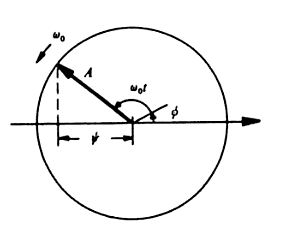
\includegraphics[width=0.5\textwidth]{Imagenes/Fasor.png}
  \caption{El fasor que genera $\psi(t)$. a $t=0$ el vector est\'a a un \'angulo $\phi$ del eje}
  \label{Fasor}
\end{figure}

Luego en el caso de querer sumar dos vibraciones $\psi = \psi_1 + \psi_2$ podemos representar el nuevo fasor de $\psi_2$ con el eje de coordenadas \textbf{en el fin del anterior}, tal como hac\'iamos con la suma de vectores. Es m\'as como cuando trabajamos en la forma polar vimos que el producto de complejos resulta en el producto de sus  m\'odulos y la suma de sus argumentos, el producto de fasores resulta en el producto de sus m\'odulos y la suma de sus fases iniciales $\phi_1+\phi_2$. 


\paragraph{Y para que sirve?} Simple, cuando tenemos una relaci\'on entre vibraciones que debe valer para todo tiempo las podemos especializar en $t=0$ por ejemplo, y podemos traducir la ecuaci\'on en fasores y de all\'i poder verificar $A$ y $\phi$ que lo cumplan para ese $t$ y por ende deben valer $\forall t$

\section{Identidades \'utiles}

Para finalizar \'esta secci\'on ser\'ia \'util presentar algunas de la identidades mas utilizadas en el trascurso del apunte y poder demostrarlas brevemente:

\begin{enumerate}
\item $\int\limits_0^{2\pi}{\cos^2(x)} \ dx = \pi$
\[
\begin{array}{rcl}
\int\limits_0^{2\pi}{\cos^2(x)} \ dx & = &  \int\limits_0^{2\pi}{\frac{1+\cos(2x)}{2}} \ dx  \\
& = & \int\limits_0^{2\pi}{\frac{1}{2}} \ dx + \int\limits_0^{2\pi}{\frac{\cos(2x)}{2}} \ dx  \\
& = & \frac{2\pi}{2} + \frac{\left({\sin(4\pi)-\sin(0)}\right)}{4}  =  \pi + 0 = \pi  
\end{array}
\]
\item $\int\limits_0^{2\pi}{\sin^2(x)} \ dx = \pi$
\item $\int\limits_0^{2\pi}{\cos(x)\sin(x)} \ dx = 0$
\[
\begin{array}{rcl}
\int\limits_0^{2\pi}{\cos(x)\sin(x)} \ dx & = & \int\limits_0^{2\pi}{\frac{\sin(2x)}{2}} \ dx \\
& = & \left(\frac{-\cos(2x)}{4}\right)\vert_{0}^{2\pi} \\
& = & \frac{1}{4}\left(\cos(0)-\cos(4\pi)\right) = 0
\end{array}
\]
\item $\left(1+\epsilon\right)^{\alpha} \approx 1 + \alpha \epsilon + \frac{\alpha(\alpha - 1)}{2}\epsilon^2 \ \ (\vert \epsilon \vert < 1)$ Donde generalmente se toma solamente el primer orden, ie: $\left(1+\epsilon\right)^{\alpha} \approx 1 + \alpha \epsilon $
\[f(\epsilon)=\left(1+\epsilon\right)^{\alpha} \ \Longrightarrow \ f(\epsilon) \approx f(0) + \frac{f'(0)}{2} + \frac{f^{\mbox{\begin{tiny}{\textit{II}}\end{tiny}}}(0)}{6} \]
\end{enumerate}


\end{document}